\documentclass[margin,line]{resume}
 
\usepackage[utf8]{inputenc}  % Changed from latin1 to utf8
\usepackage[french]{babel}
\usepackage[T1]{fontenc}
\usepackage{fontawesome}
\usepackage{graphicx,wrapfig}
\usepackage{url}
\usepackage[colorlinks=true, pdfstartview=FitV, linkcolor=blue, citecolor=blue, urlcolor=blue]{hyperref}
\ifdefined\pdfcompresslevel
\pdfcompresslevel=9
\fi


\begin{document}{\sc \Large Curriculum Vitae -- Arthur Guiot}
\begin{resume}

% === PICTURE ===

    \vspace{0.3cm}
    \begin{wrapfigure}{R}{0.15\textwidth}
         \vspace{-1.5cm}
        \begin{center}
        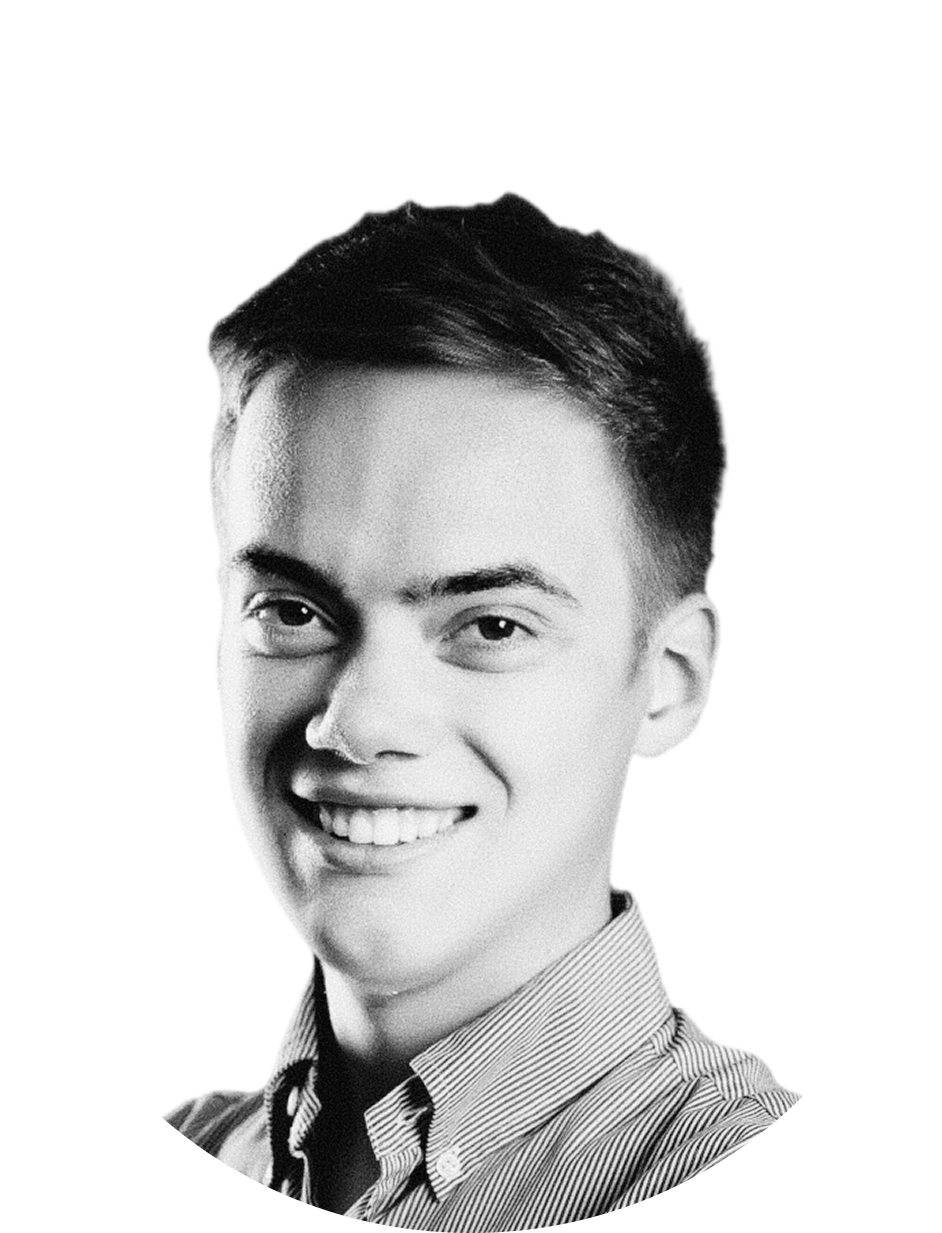
\includegraphics[width=0.15\textwidth]{profile_picture.png}
        \end{center}
         \vspace{-1cm}
    \end{wrapfigure}

% === PERSONAL INFO ===
 
    \section{\mysidestyle Informations\\Personnelles}
    Arthur Guiot \\
    Santa Clara, Californie, États-Unis \\ 
    \faPhone \space +1 (863) 210-4074 \\
    \faEnvelope \space \href{mailto:arguiot@gmail.com}{arguiot@gmail.com} \\ 
    \faGlobe \space \href{https://arguiot.com}{arguiot.com} \\ 
    \faGithub \space \href{https://github.com/arguiot}{github.com/arguiot} \\
    Contributeur actif à l'open-source avec plus de 7 500 contributions et 2 000+ stars sur GitHub
   
% === OBJECTIVE ===

    \section{\mysidestyle Objectif Professionnel}
    Étudiant en génie logiciel avec 8 ans d'expérience en développement d'applications, optimisation de sites web et technologie blockchain. Cherche à mettre à profit son expertise technique dans le développement d'applications financières haute performance et de systèmes distribués pour stimuler l'innovation dans les secteurs de la technologie et de la finance.
 
% === SKILLS ===
       
    \section{\mysidestyle Compétences}\vspace{2mm}       
    \begin{description}
        \item[User Facing:] Next.js, Tailwind, React, SwiftUI, UIKit, AppKit
        \item[Business Logic:] TypeScript, Python, Swift, C \& C++, SQL, Solidity, Rust
        \item[Technologies:] Git, Linux, AWS, Kubernetes, DevOps, Docker
        \item[Autres Compétences:] Leadership, Project Management, Communication Client, Fund raising
        \item[Langues:] Français, Anglais
    \end{description}
     
% === FEATURED PROJECTS ===
    
    \section{\mysidestyle Projets Principaux}
    \begin{list2}
        \item \textbf{Euclid Calculator}\\
        Une calculatrice entièrement repensée pour macOS et iOS avec une note de 4,5 étoiles dans plusieurs pays. Recommandée par SetApp, avec plus de 50 000 téléchargements payants sur toutes les plateformes.
        \vspace{1mm}
        \item \textbf{Ultrahuman}\\
        Un système de support entièrement autonome qui aide à déboguer les tickets en lançant des agents pour inspecter les codebases et les systèmes, accélérant l'analyse des causes racines.
        \vspace{1mm}
        \item \textbf{Portfolio Manager}\\
        Système de gestion automatique de portefeuille crypto qui est passé de 0 à 100 000 \$ d'AUM en trois mois après son déploiement. Dispose de capacités étendues de backtesting pour les modèles financiers et quantitatifs au service de centaines de clients.
    \end{list2}

% === EDUCATION ===

\section{\mysidestyle Formation} 
\textbf{Santa Clara University, Californie} \hfill \textsl{Septembre 2023-Juin 2025}\\
Bachelor of Computer Science\\
\vspace{1mm}
\textbf{Florida Polytechnic University, Floride} \hfill \textsl{Janvier 2021-Septembre 2023}\\
Bachelor of Computer Science (transfert à SCU)
    
% === EMPLOYMENT HISTORY ===

    \section{\mysidestyle Expérience Professionnelle}\vspace{2mm}   	   
       
    \begin{description} 
        \item[Software Engineer]\small{Circleback \hfill \textsl{Juillet 2026-Présent}}\\
        Réalisations:
        \begin{list2}
            \item{Travail à temps plein chez Circleback, une entreprise YC développant des notes de réunion alimentées par l'IA}
            \item{Développe des produits aidant les équipes à capturer, organiser et exploiter leurs conversations de réunion plus efficacement}
            \item{Contribue au développement produit pour des workflows IA et des outils de productivité liés aux réunions}
        \end{list2}
        \vspace{2mm}

        \item[Blockchain Engineer]\small{EveryFinance \hfill \textsl{Janvier 2024-Mars 2025}}\\
        Réalisations:
        \begin{list2}
            \item{Construit des outils financiers et un framework de backtesting générant 85\% APR (moyenne sur 5 ans) pour le portfolio Alpha}
            \item{Réduit les temps de processing de 5-15 secondes à 1-3 secondes, et amélioré l'UX}
            \item{Centralisé l'état de l'infrastructure sur plus de 20 microservices et implémenté un système CI}
        \end{list2}   	
        \vspace{2mm}
 				
        \item[Blockchain Engineer Intern]\small{PyratzLabs \hfill \textsl{Mai 2023-Août 2023}}\\
        Réalisations:
        \begin{list2}
            \item{Conçu et développé un arbitrage bot avec des profits théoriques potentiels de 75 ETH par semaine selon des recherches internes}
            \item{Travaillé sur un outil d'optimisation de portefeuille guidant les décisions de stratégie d'investissement}
            \item{Contribué au développement de Securd, un protocole révolutionnaire de lending \& borrowing sur les chaînes Ethereum}
        \end{list2}  	      
        \vspace{2mm}
    \end{description}
    
\end{resume}   
\end{document}
